% Declaración de variables globales
% imagnes de las metricas
\newcommand{\metrica}{../img/metricas/1.png}
\newcommand{\metricas}{../img/metricas/2.png}




\section{METRICAS}
\subsection{Métricas indirectas – Métricas orientadas a la función}
\subsubsection{Rask.ai}

\begin{doublespace} 

Rask.ai es una herramienta fantástica de localización que puede traducir vídeos
a más de 60 idiomas de forma eficaz. Además, con sus tecnologías "Texto-a voz" y
"Clonación de voz", puedes añadir una voz en off que suene natural sin necesidad de
contratar a un actor de doblaje \par

Lo que hace esta IA no es solo doblar una voz a cualquier idioma, sino mantener
cómo suena la voz, para que parezca que es esa misma persona la que está hablando
en otro idioma.\par

El proceso de creación de estas plataformas de traducción consta de cuatro
partes, primero, el paso de voz a texto, al que le sigue la traducción y, después, una de
las partes más complejas: pasar del texto traducido con un tono de voz muy parecido al
original. Por último, se procesa la imagen para que el movimiento de los labios
corresponda con la aplicación.\par

La aplicación analiza el texto que forma para el vídeo para después poder
traducirlo de forma inmediata. No sólo eso, sino que analiza la tonalidad y el tipo de
voz de la persona que esté hablando y consigue mantenerlas.\par


Puede ayudar para ver cómo sería tu pronunciación en un idioma o a utilizarte a
ti mismo de modelo y observes cómo debes pronunciar. Incluso te puede salvar si
necesitas comunicarte con alguien de otro idioma del cual no tienes ningún tipo de
formación.\par

Otros usos importantes son: la formación de empleados/as y clientes, marketing,
creación y distribución de contenidos, videos educativos, desarrollo en videojuegos o
vídeos de ventas entre otros. (Rask, 2023)\par\vspace{0.3cm}

\centering
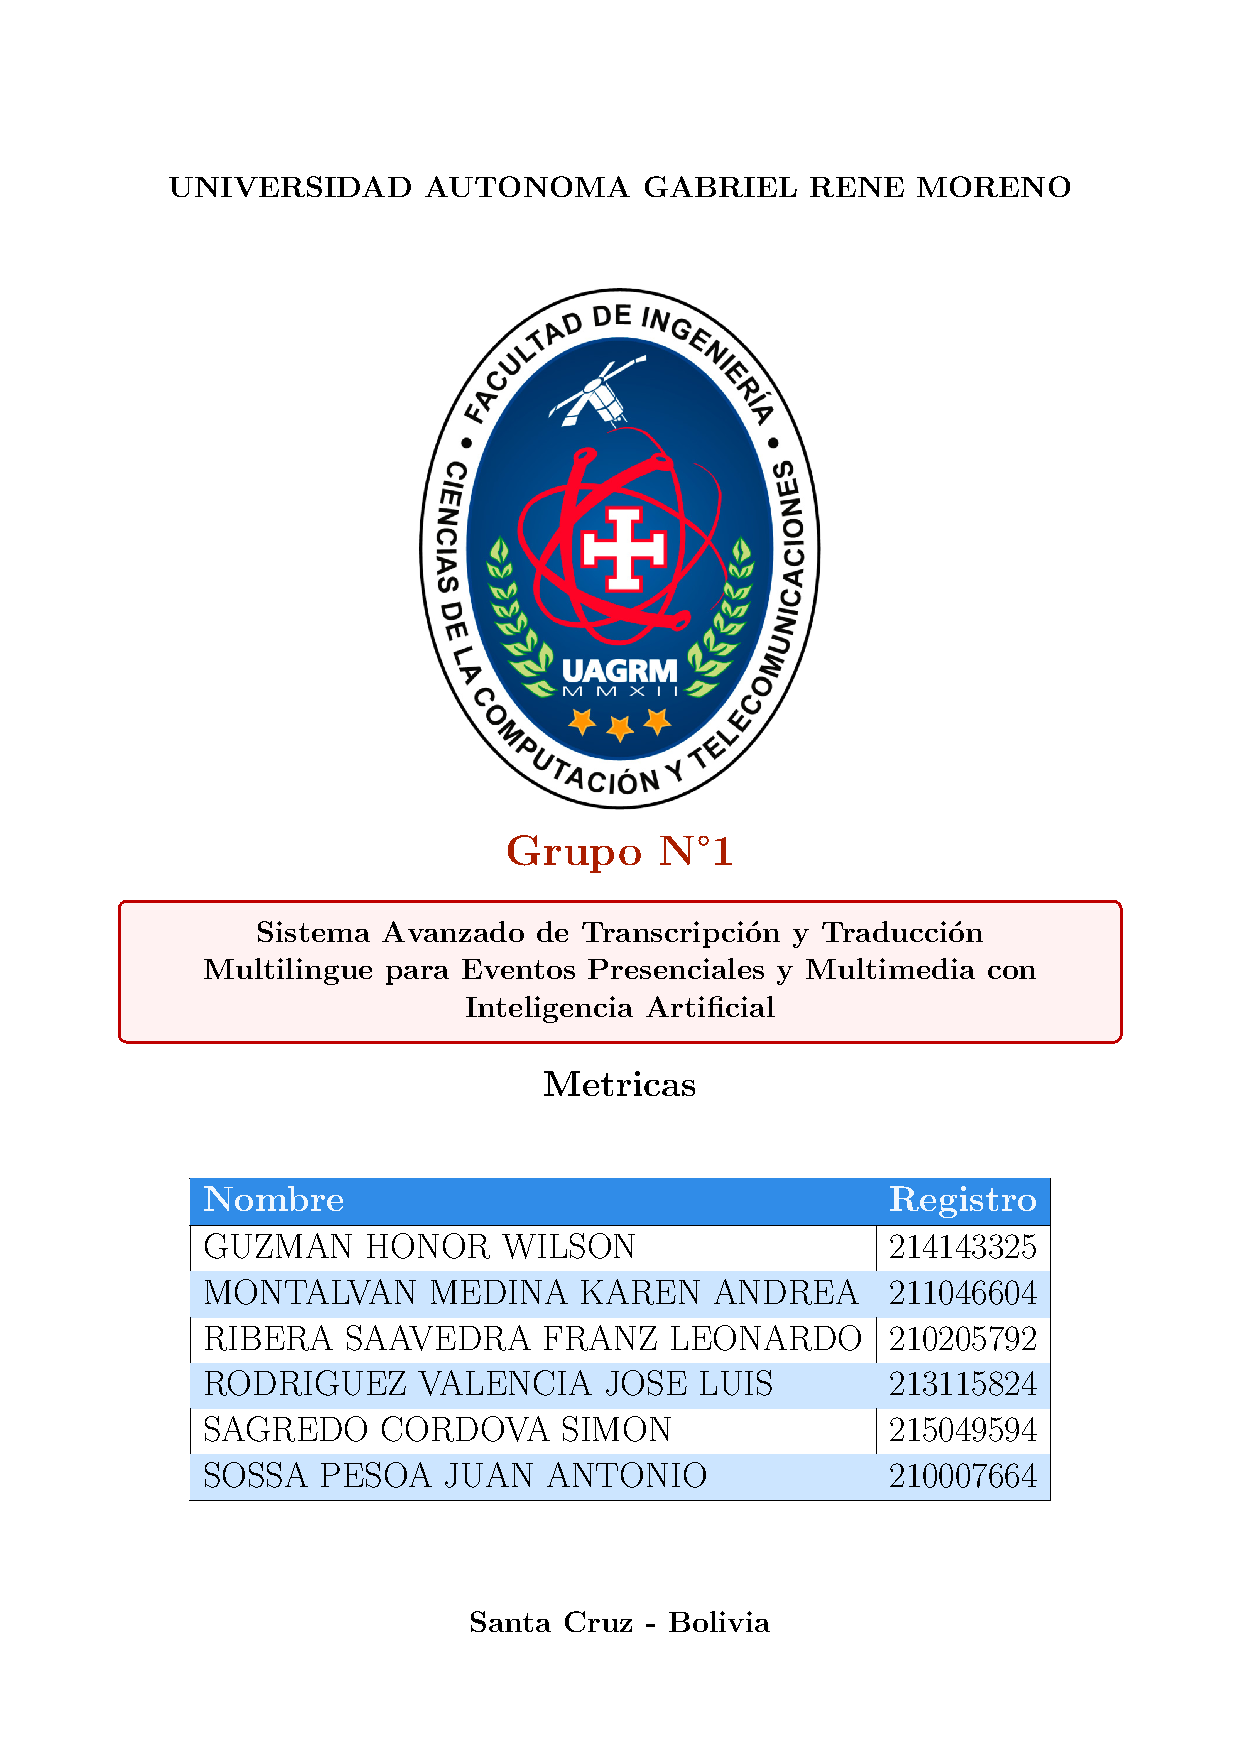
\includegraphics[width=0.8\textwidth]{\metrica}\par\vspace{0.3cm}
Ilustración 1: Interfaz de Rask.ai



\centering
\includegraphics[width=0.8\textwidth]{\metricas}\par\vspace{0.3cm}
Ilustración 2: Interfaz de Rask.ai


\clearpage  %nueva pagina
\subfile{indirecta/m_indirecta_rask.tex}


\clearpage  %nueva pagina

\end{doublespace}